\documentclass[11pt]{article}

\usepackage[margin=1in]{geometry}
\usepackage{amsmath, amssymb}
\usepackage{booktabs}
\usepackage{hyperref}
\usepackage{enumitem}
\usepackage{tikz}
\usetikzlibrary{arrows.meta, positioning}

\title{Training \texttt{SimpleDiTWorldModel}: A Distilled World Model for MPC}
\author{}
\date{}

\begin{document}
\maketitle

\section{Motivation}

\texttt{simple\_dit\_bc}'s BC policy (\texttt{SimpleDiTBC}, described separately) can only propose
an action chunk -- it cannot evaluate a candidate action chunk before executing it. The full Cosmos
Policy model \emph{can}: its own best-of-N planner samples $N$ candidate action chunks, imagines
each one's future state and value with the 2B-parameter teacher, and executes only the
best-scoring candidate. This works well but is expensive -- every planning step costs several
diffusion-sampling passes through a cross-attention DiT plus a VAE decode, for each candidate.

\texttt{SimpleDiTWorldModel} is a small model, architecturally a sibling of \texttt{SimpleDiTBC}
(same conv+spatial-softmax image encoder, same AdaLN-conditioned transformer-block design), trained
to answer the same question -- ``given this state and this candidate action, what happens, and how
good is it?'' -- cheaply enough to run inside a best-of-N loop many times per control step. Its
dynamics/value knowledge is \emph{distilled} from the already-trained 2B teacher rather than
learned from demonstration data alone, for a specific reason: a value model trained only on the
recorded (on-trajectory) actions in the demos never sees the off-trajectory candidate actions a
best-of-N search proposes, and has no reason to generalize to scoring them. The teacher can be
queried on \emph{any} action, including ones no demonstrator ever took, so its predictions there
are exactly the training signal the small model needs.

\section{Training Data: Real and Synthetic Branches}

Every training sample is a tuple
$(\text{agentview}_t, \text{wrist}_t, \text{proprio}_t, a_{t:t+H}, e_{\text{task}}, \text{agentview}_{t+K}, \text{wrist}_{t+K}, v)$
-- current observation, a candidate $H$-step action chunk, and the resulting future observation and
scalar value $H=K=$ \texttt{chunk\_size} steps later. Two disjoint sources fill this format:

\subsection{Real samples (no teacher needed)}

For every $(episode, t)$ in the demo data, the \emph{recorded} action chunk actually executed by
the demonstrator is paired with the \emph{real} frame at $t+K$ (clipped to the episode's last frame
if it ends first) and a real Monte-Carlo return-to-go over the demo's sparse terminal-success
reward ($r_\tau = 1$ at $\tau=T-1$, $0$ otherwise, since every demo here is a successful episode):
\begin{equation}
    v_t = \sum_{k=0}^{T-t-1} \gamma^k r_{t+k} = \gamma^{\,T-1-t} \in [0, 1],
\end{equation}
monotonically approaching $1$ as $t \to T-1$. (\texttt{compute\_monte\_carlo\_returns} internally
rescales this to $[-1,1]$ to match the teacher's own value-prediction convention before it's
rescaled back to $[0,1]$ for the cache -- a round trip that is the identity when the terminal
reward is exactly $1$, as it is here, so $v_t = \gamma^{T-1-t}$ directly.) This branch requires
nothing beyond what's already loaded into memory for BC training -- it is exactly as cheap to
compute as the action-chunk target already is.

\subsection{Synthetic samples (teacher-imagined counterfactuals)}

For a sampled subset of $(episode, t)$, the recorded action chunk is perturbed with Gaussian noise
in normalized action space,
\begin{equation}
    \tilde{a}_{t:t+H} = \operatorname{clip}\!\big(a_{t:t+H} + \epsilon,\ -1,\ 1\big), \qquad
    \epsilon \sim \mathcal{N}(0, \sigma^2 I),
\end{equation}
producing a candidate action the demonstrator never took. This candidate is scored by the frozen
2B teacher (\texttt{nvidia/Cosmos-Policy-LIBERO-Predict2-2B}) via a three-step query:
\begin{enumerate}[nosep]
    \item Query the teacher's action head once to obtain a valid conditioning latent
    (\texttt{get\_action}), discarding its own sampled action.
    \item \textbf{Inject} the perturbed candidate $\tilde{a}_{t:t+H}$ directly into that latent's
    action slot, overwriting the teacher's own sample -- the one piece of new machinery this
    pipeline needed, since the teacher has no built-in interface for evaluating a
    caller-supplied action.
    \item Re-run the teacher's future-state and value heads
    (\texttt{get\_future\_state\_prediction}, \texttt{get\_value\_prediction}) conditioned on the
    injected latent, yielding an imagined future frame pair and a scalar value estimate
    $\tilde{v} \in [0,1]$ for the counterfactual action.
\end{enumerate}
The teacher's decoded future frames (natively $224\times224$) are resized down to the student's
$96\times96$ resolution before being cached. This branch is what gives the student exposure to the
broader action distribution a best-of-N sampler will actually query at inference time -- coverage
the real branch alone cannot provide.

\section{Training Objective}

Unlike \texttt{SimpleDiTBC}'s rectified-flow objective, \texttt{SimpleDiTWorldModel} is trained
with \emph{direct MSE regression}: there is no distributional-multimodality concern for a value
scalar or a future-frame embedding the way there is for actions (many actions can plausibly follow
a given state, but a given \emph{state-action pair} has one predicted outcome), so no
noise/timestep input or iterative sampling is needed at either train or inference time --- a single
forward pass suffices.

The model outputs a predicted future-agentview embedding, future-wrist embedding (each
$\in \mathbb{R}^{256}$, matching \texttt{SmallImageEncoder}'s pre-projection spatial-softmax
feature dimension), and a scalar value:
\begin{equation}
    (\hat{f}_{\text{agent}},\ \hat{f}_{\text{wrist}},\ \hat{v}) =
    f_\theta(\text{agentview}_t, \text{wrist}_t, \text{proprio}_t, a_{t:t+H}, e_{\text{task}}).
\end{equation}
The regression targets for the two embeddings are \emph{not} precomputed and frozen -- they are
produced at each training step by encoding the target future frames with the model's \emph{own}
(currently-being-trained) \texttt{SmallImageEncoder}, under \texttt{no\_grad}:
\begin{equation}
    f_{\text{agent}} = \text{SmallImageEncoder}(\text{agentview}_{t+K})_{\text{pre-proj}}, \qquad
    f_{\text{wrist}} = \text{SmallImageEncoder}(\text{wrist}_{t+K})_{\text{pre-proj}}.
\end{equation}
This keeps the target space consistent with whatever the encoder currently represents (rather than
a stale snapshot from a different checkpoint), and lets real and teacher-imagined future frames
share one target-encoding pipeline. The loss is the sum of three MSE terms:
\begin{equation}
    \mathcal{L}(\theta) = \big\| \hat{f}_{\text{agent}} - f_{\text{agent}} \big\|_2^2
        + \big\| \hat{f}_{\text{wrist}} - f_{\text{wrist}} \big\|_2^2
        + \big( \hat{v} - v \big)^2.
\end{equation}

\subsection{Optimization}

Identical scaffolding to \texttt{SimpleDiTBC}'s training recipe: AdamW with linear warmup then
cosine decay to a floor of \texttt{min\_lr\_ratio} $\times$ peak learning rate, and the same
pad-crop/brightness/contrast image augmentation applied to the \emph{current-state} images (not
the future-target images, which are held fixed as regression targets).

\section{Architecture Summary}

\texttt{SimpleDiTWorldModel} conditions on current state \emph{and} the candidate action being
evaluated, then refines three fixed learned query tokens (future-agentview, future-wrist, value)
through the same AdaLN-Zero \texttt{DiTBlock} stack \texttt{SimpleDiTBC} uses over action tokens:
\begin{equation}
    c = \text{vision\_combiner}(e_{\text{agent}}, e_{\text{wrist}})
        + \text{MLP}_{\text{proprio}}(\text{proprio}_t)
        + \text{MLP}_{\text{task}}(e_{\text{task}})
        + \text{MLP}_{\text{action}}(a_{t:t+H}),
\end{equation}
where $\text{MLP}_{\text{action}}$ (\texttt{ActionChunkEncoder}) flattens and projects the
candidate action chunk into the conditioning space -- the only architectural addition relative to
\texttt{SimpleDiTBC}'s encoders. Each of the three output tokens is projected back to its target
dimension (256, 256, 1) by its own small \texttt{FinalLayer} head, since the three targets have
different dimensionalities and a single shared head would need extra padding/masking machinery
for no real benefit.

\section{How Close Is This to the Full Cosmos Policy Model?}

\texttt{SimpleDiTWorldModel} is not a smaller version of the teacher's architecture -- it is a
different architecture entirely, trained only to match the teacher's \emph{input/output contract}
(state, candidate action $\to$ future state, value) closely enough that \texttt{eval\_mpc.py}'s
best-of-N search can call either one interchangeably. Table~\ref{tab:teacher-vs-student} makes the
gap concrete.

\begin{table}[h]
\centering
\begin{tabular}{@{}lll@{}}
\toprule
& \textbf{Teacher (Cosmos-Policy-*-Predict2-2B)} & \textbf{Student (\texttt{SimpleDiTWorldModel})} \\
\midrule
Parameters & $\sim 2$B & $8.56$M ($\sim$235$\times$ smaller) \\
Visual repr. & VAE latent (\texttt{tokenizer.encode}) & raw RGB $\to$ conv + spatial-softmax \\
Text conditioning & cross-attn.\ over 512 T5 tokens & one pooled T5 vector, summed via AdaLN \\
Token mixing & self+cross-attn.\ DiT (WAN-style) & self-attn.\ only, 3 fixed query tokens \\
Inference & multi-step denoising + VAE decode & single deterministic forward pass \\
Image resolution & $224\times224$, decoded to pixels & $96\times96$, never decoded (feature-only) \\
Future-state output & decoded RGB frame(s) & 256-d pre-projection encoder feature \\
Value output & read from a latent index in the & dedicated scalar head \\
& same video latent as the action/state & \\
\bottomrule
\end{tabular}
\caption{Teacher/student comparison. Denoising-step counts above are this pipeline's own defaults
(\texttt{num\_denoising\_steps\_action=5}, \texttt{=\_future\_state=1}, \texttt{=\_value=1} in
\texttt{precompute\_teacher\_targets.py}); the teacher supports more steps at higher quality/cost.}
\label{tab:teacher-vs-student}
\end{table}

What \emph{is} shared: the teacher packs current state, action, future state, and value into one
spatiotemporal video latent and reads each quantity off a different latent index of a single
generative model -- so one query already answers all three questions at once. The student mirrors
that shape structurally (one conditioning vector, three output heads refined together through the
same block stack) without sharing any of the underlying machinery that produces it.

What is \emph{not} yet known is the empirical fidelity of the distillation -- i.e.\ how well the
student's future-state features and value actually agree with the teacher's on held-out
counterfactual actions. \texttt{precompute\_teacher\_targets.py} has not been run against a real
GPU yet (see its own module docstring), so the $\sim$235$\times$ parameter reduction above is
presently a design target, not a measured result: there are no teacher/student agreement numbers
(e.g.\ value correlation, future-feature MSE against a teacher held out at eval time) to report.
That validation is the natural next step once a synthetic cache and a trained checkpoint both
exist.

\subsection{Pipeline Diagrams}

Figures~\ref{fig:teacher-arch} and~\ref{fig:student-arch} lay out both pipelines top to bottom.
Orange boxes are steps that exist on \emph{one} side only -- gray boxes are the part of the recipe
(AdaLN-Zero-modulated self-attention blocks) both models actually share.

\begin{figure}[h]
\centering
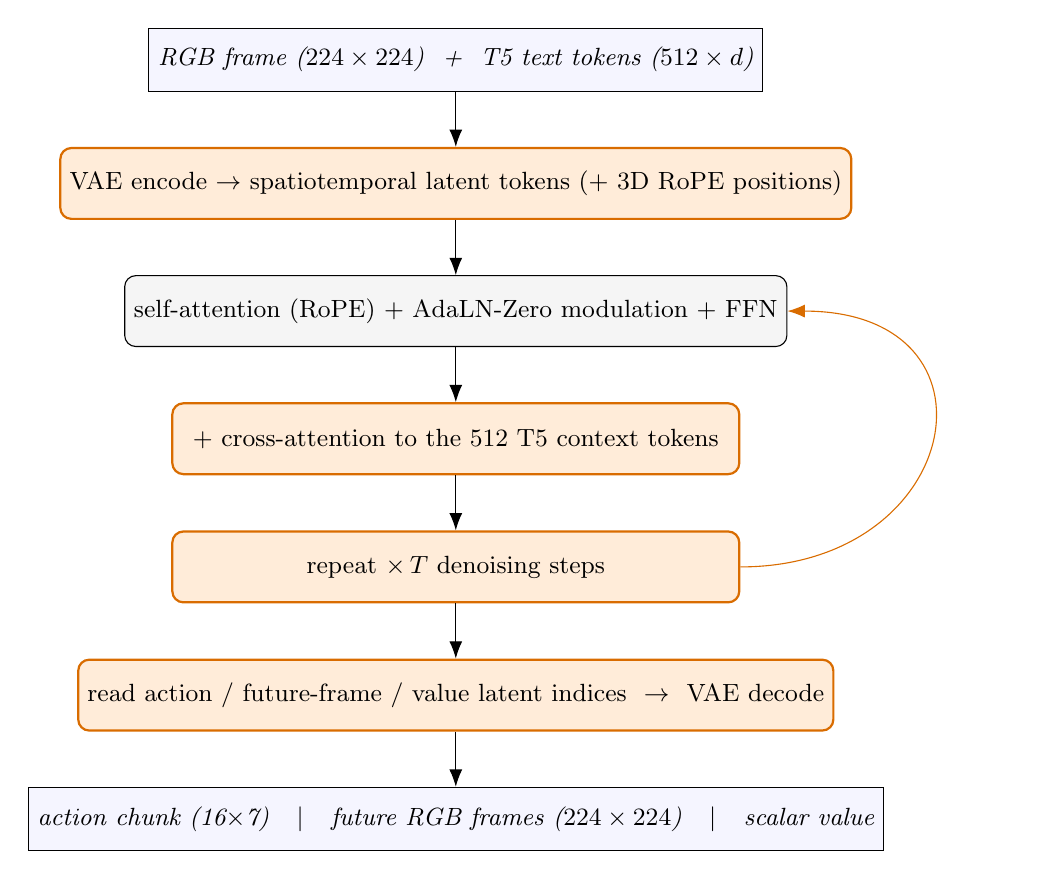
\begin{tikzpicture}[
  node distance=7mm,
  block/.style={draw, rounded corners, align=center, minimum width=7.2cm, minimum height=0.9cm, fill=gray!8, font=\small},
  diff/.style={draw=orange!85!black, thick, rounded corners, align=center, minimum width=7.2cm, minimum height=0.9cm, fill=orange!15, font=\small},
  io/.style={draw, align=center, minimum width=7.2cm, minimum height=0.8cm, fill=blue!4, font=\small\itshape},
  arr/.style={-{Latex[length=2.2mm]}}
]
\node[io]   (t1) {RGB frame ($224\times224$) \ + \ T5 text tokens ($512\times d$)};
\node[diff, below=of t1] (t2) {VAE encode $\to$ spatiotemporal latent tokens (+ 3D RoPE positions)};
\node[block, below=of t2] (t3) {self-attention (RoPE) + AdaLN-Zero modulation + FFN};
\node[diff, below=of t3] (t4) {+ cross-attention to the 512 T5 context tokens};
\node[diff, below=of t4] (t5) {repeat $\times\, T$ denoising steps};
\node[diff, below=of t5] (t6) {read action / future-frame / value latent indices \ $\to$ \ VAE decode};
\node[io,   below=of t6] (t7) {action chunk (16$\times$7) \ \ $\vert$ \ \ future RGB frames ($224\times224$) \ \ $\vert$ \ \ scalar value};

\draw[arr] (t1) -- (t2);
\draw[arr] (t2) -- (t3);
\draw[arr] (t3) -- (t4);
\draw[arr] (t4) -- (t5);
\draw[arr, orange!85!black] (t5.east) to[out=0, in=0, looseness=2.2] (t3.east);
\draw[arr] (t5) -- (t6);
\draw[arr] (t6) -- (t7);
\end{tikzpicture}
\caption{Teacher (\texttt{Cosmos-Policy-*-Predict2-2B}) pipeline. The looped arrow on the right is
the multi-step denoising iteration -- every step re-enters the same DiT stack.}
\label{fig:teacher-arch}
\end{figure}

\begin{figure}[h]
\centering
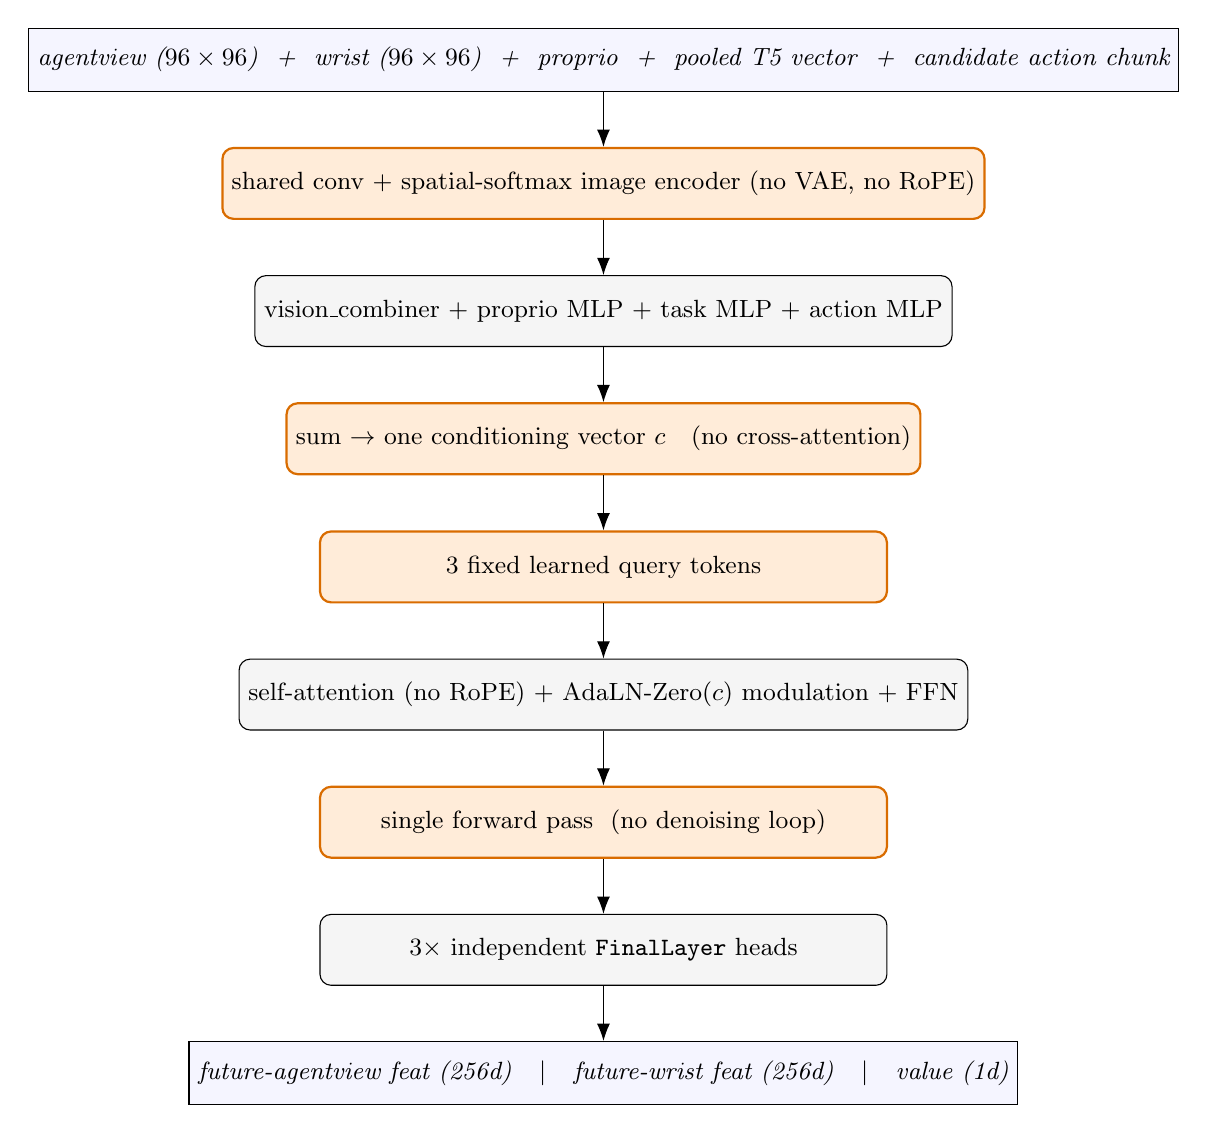
\begin{tikzpicture}[
  node distance=7mm,
  block/.style={draw, rounded corners, align=center, minimum width=7.2cm, minimum height=0.9cm, fill=gray!8, font=\small},
  diff/.style={draw=orange!85!black, thick, rounded corners, align=center, minimum width=7.2cm, minimum height=0.9cm, fill=orange!15, font=\small},
  io/.style={draw, align=center, minimum width=7.2cm, minimum height=0.8cm, fill=blue!4, font=\small\itshape},
  arr/.style={-{Latex[length=2.2mm]}}
]
\node[io]   (s1) {agentview ($96\times96$) \ + \ wrist ($96\times96$) \ + \ proprio \ + \ pooled T5 vector \ + \ candidate action chunk};
\node[diff, below=of s1] (s2) {shared conv + spatial-softmax image encoder (no VAE, no RoPE)};
\node[block, below=of s2] (s3) {vision\_combiner + proprio MLP + task MLP + action MLP};
\node[diff, below=of s3] (s4) {sum $\to$ one conditioning vector $c$ \ \ (no cross-attention)};
\node[diff, below=of s4] (s5) {3 fixed learned query tokens};
\node[block, below=of s5] (s6) {self-attention (no RoPE) + AdaLN-Zero($c$) modulation + FFN};
\node[diff, below=of s6] (s7) {single forward pass \ (no denoising loop)};
\node[block, below=of s7] (s8) {3$\times$ independent \texttt{FinalLayer} heads};
\node[io,   below=of s8] (s9) {future-agentview feat (256d) \ \ $\vert$ \ \ future-wrist feat (256d) \ \ $\vert$ \ \ value (1d)};

\draw[arr] (s1) -- (s2);
\draw[arr] (s2) -- (s3);
\draw[arr] (s3) -- (s4);
\draw[arr] (s4) -- (s5);
\draw[arr] (s5) -- (s6);
\draw[arr] (s6) -- (s7);
\draw[arr] (s7) -- (s8);
\draw[arr] (s8) -- (s9);
\end{tikzpicture}
\caption{Student (\texttt{SimpleDiTWorldModel}) pipeline. Same self-attn/AdaLN-Zero block core as
the teacher (gray), everything orange is either simplified away or replaced.}
\label{fig:student-arch}
\end{figure}

\end{document}
